%!TEX root = skripsi.tex
%-----------------------------------------------------------------------------%
\chapter{\babEmpat} \label{implementasi}
%-----------------------------------------------------------------------------%
Bab ini akan menjelaskan perihal implementasi dari pemindahan \textit{sense} dan sistem \textit{WSD} yang dibuat.


\section{Peningkatan Kualitas \textit{Alignment}}

\begin{lstlisting}[language=Python, caption={Word Alignment Enhancement}, label={word-alignment-enhancement}]

dict_id = {}
dict_en = {}

# masukan setiap kosa kata bahasa Indonesia ke dalam dict_id sebagai key dan kumpulan pasangan kata bahasa inggrisnya sebagai value
# proses yang sama dilakukan untuk dict_en dengan kosa kata bahasa Inggris sebagai key dan kumpulan pasangan kata bahasa Indonesia sebagai value
# stop adalah list stopword yang didapat dari korpus nltk

# this section is for filtering which english word that has corresponding indo translation (bidirectional) from Giza output
for indo_word in dict_id.keys():
if indo_word not in dict_en:
# filtering so no same translation is entered, answer -> answer, jawaban -> jawaban
for en_word in dict_id[indo_word].keys():
if en_word in dict_en and indo_word in dict_en[en_word] and en_word not in stop:
if indo_word not in final_dictionary:
final_dictionary[indo_word] = { en_word: dict_en[word_en][word_id] }
else:
if en_word not in final_dictionary[indo_word]:
final_dictionary[indo_word][en_word] = dict_en[word_en][word_id]
\end{lstlisting}

%-----------------------------------------------------------------------------%
\section{Sistem WSD}
Sistem WSD dibangun dengan menggunakan \textit{supervised learning}. Pada sistem ini terdapat dua buah bagian utama yaitu pemilihan fitur serta \textit{classifier} dan evaluasi hasil \textit{classifier}.

\subsection{Pemilihan Fitur dan \textit{Classifier}}
Terdapat n buah fitur pada penelitian ini yang terdiri dari:

\begin{enumerate}
	\item Fitur \textit{bag of words} yang merupakan kata samping kanan dan kiri dengan \textit{window} sebanyak dua buah kata
	\item Fitur \textit{POS tagging}
	\item Vektor dari hasil \textit{word embedding}
\end{enumerate}

\textit{Classifier} yang digunakan pada penelitian ini adalah SVM dengan \textit{library} Python yaitu Scikit dengan parameter \textit{default} berupa kernel linear dan C=1.

\subsection{Evaluasi Sistem}
Evaluasi dilakukan dengan \textit{cross validation} menggunakan perhitungan rata-rata akurasi dari hasil klasifikasi yang dilakukan \textit{classifier}. \textit{Crossvalidation} dilakukan dengan interasi sebanyak tiga buah.

%-----------------------------------------------------------------------------%
\section{Ekstraksi Teks}
%-----------------------------------------------------------------------------%
Hal pertama yang harus dilakukan terhadap berkas XML Wikipedia adalah membersihkan berkas tersebut dari format Wiki \textit{markup language}. Ekstraksi dilakukan dengan bantuan \textit{tools} Wikipedia Extractor\footnote{http://medialab.di.unipi.it} yang berupa program berbahasa Python untuk mengekstrak dan membersihkan dokumen XML Wikipedia. Program ini dibuat oleh Giuseppe Attardi dan Antonio Fuschetto dari University of Pisa, Italia, dan telah direvisi oleh beberapa kontributor. 

Untuk membersihkan berkas XML semua artikel Wikipedia, \textit{tools} Wikipedia Extractor bisa langsung dijalankan dengan perintah berikut pada terminal.

\begin{lstlisting}
WikiExtractor.py [nama berkas masukan] -o [nama berkas keluaran]
\end{lstlisting}

\begin{figure}
	\centering
	\includegraphics[width=1\linewidth]{pics/wiki-XML-2}
	\caption{Potongan artikel pada berkas XML Wikipedia}
	\label{fig:wiki-XML}
\end{figure}
Gambar \ref{fig:wiki-XML} menunjukkan potongan isi berkas masukan yang berupa XML semua artikel Wikipedia. Sedangkan, gambar \ref{fig:hasil-ekstraksi} menunjukkan hasil yang dikeluarkan program Wikipedia Extractor setelah melakukan ekstraksi pada potongan isi artikel di gambar \ref{fig:wiki-XML}.
\begin{figure}
	\centering
	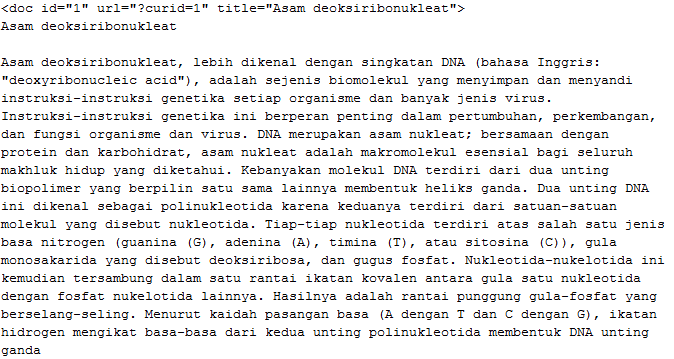
\includegraphics[width=1\linewidth]{pics/hasil-ekstraksi}
	\caption{Hasil Ekstraksi pada XML seluruh artikel Wikipedia}
	\label{fig:hasil-ekstraksi}
\end{figure}
\noindent Setelah melalui proses ekstraksi, hanya teks di dalam \textit{tag} \textit{text} saja yang diambil dan dibersihkan. Format Wikipedia \textit{markup language} yang dibersihkan, antara lain dengan penghapusan tabel dan gambar (teks di dalam kotak biru pada gambar \ref{fig:wiki-XML}), serta pembersihan format \textit{hyperlink} (teks yang diberi garis merah pada gambar \ref{fig:wiki-XML}).

\textit{Tools} Wikipedia Extractor hanya menerima struktur XML semua artikel Wikipedia, sehingga tidak dapat mengolah XML Wikipedia \textit{revision history}. Oleh karena itu, ada sedikit variasi yang dilakukan agar tetap bisa menggunakan \textit{tools} ini pada data Wipedia \textit{revision history}. Variasi tersebut ditunjukkan pada kode \ref{ekstraksi-wiki-rev}. 

\begin{lstlisting}[language=Python, caption={Ekstraksi Wikipedia Revision History}, label={ekstraksi-wiki-rev}]
#Sediakan berkas template XML artikel Wikipedia yang kosong
template = #berkas template XML artikel Wikipedia
revision = #berkas XML Wikipedia Revision History

for page in revision: #semua artikel 
	page_revision = []
	page_id = #id artikel
	for r in page: #semua teks revisi 
		comment = #teks di dalam tag comment
		r_id = #id teks revisi
		p_id = #id induk teks revisi
		#masukan teks revisi ke dalam template XML
		template.insert_text(r)
		#panggil program WikiExtractor dan ekstrak template
		extracted = run_command(WikiExtractor.py template)
		page_revision.add([extracted, comment, r_id, p_id])
		#bersihkan teks template
		template.clear()
	#cetak page_revision
\end{lstlisting}
Berdasarkan kode \ref{ekstraksi-wiki-rev}, isi dari artikel Wikipedia \textit{revision history} pada setiap versi revisi dimasukkan ke dalam \textit{template} yang memiliki struktur serupa dengan Wikipedia \textit{all article}. Kemudian, \textit{template} yang sudah diganti isinya diekstrak menggunakan \textit{tools} Wikipedia Extractor dan disimpan hasil keluarannya bersama dengan beberapa informasi lain yang dibutuhkan, seperti informasi di dalam \textit{tag comment} dan \textit{id}. Setelah program ini dijalankan, hasil yang diperoleh akan seperti contoh pada gambar \ref{fig:revisi_induk}. 

%-----------------------------------------------------------------------------%
\section{Pemisahan kalimat}
%-----------------------------------------------------------------------------%
Hasil ekstraksi Wikipedia seluruh artikel dipisahkan menjadi kalimat per kalimat, lalu masing-masing kalimat dilakukan normalisasi. Dalam sebuah teks, kalimat dipisahkan dengan menggunakan tanda baca titik, seru, dan tanya. Namun ada beberapa kondisi khusus yang menunjukkan bahwa kemunculan tanda tersebut bukan berarti sebagai pemisah kalimat, yaitu:
\begin{enumerate}
	\item Kemunculan tanda baca berada di dalam suatu kutipan dan  tanda kurung. Contoh: "Pertumbuhan penjualan tahun ini (lihat Tabel 9.1) menunjukkan kenaikan yang pesat.".
	
	\item Kemunculan tanda baca berada dalam suatu istilah (seperti alamat situs) atau bilangan. Contoh: istilah www.google.com dan bilangan 1.000.000.
	
	\item Kemunculan tanda baca berada dalam sebuah singkatan umum Indonesia atau sebuah gelar. Contoh: dll., dsb., tgl., hlm., S.Kom., S.Pd., Dr.
\end{enumerate}
Pada tahap ini juga dilakukan normalisasi. Ada dua jenis normalisasi yang dilakukan, yaitu normalisasi gelar dan singkatan serta normalisasi tanda baca. 
\begin{enumerate}
	\item Normalisasi gelar dan singkatan. \\Normalisasi ini dilakukan untuk kata-kata yang mengandung tanda baca titik di dalamnya, seperti singkatan dan gelar. Kata-kata tersebut rawan mengalami kesalahan penulisan, misalnya "S.Kom." ditulis "S.Kom" atau juga singkatan seperti "dll." ditulis "dll" (tanpa titik). Untuk mengimplementasikan normaliasasi ini, kemungkinan-kemungkinan bentuk kesalahan penulisan yang umum terjadi didaftarkan terlebih dahulu. Kemudian tiap kesalahan tersebut dipetakan pada penulisan yang benar.
	
	\item Normalisasi tanda baca \\Kalimat-kalimat yang terbentuk kemudian mengalami normalisasi tanda baca, yaitu pemisahan tanda baca yang menempel pada kata-kata di kalimat kecuali kata yang memang mengandung tanda baca tersebut (tidak memiliki arti jika tidak dengan tanda baca, contohnya singkatan, gelar, alamat situs). Contoh kalimat yang sudah mengalami normalisasi tanda baca:
	"Chairil meninggal dalam usia muda di Rumah Sakit CBZ ( sekarang Rumah Sakit Dr. Cipto Mangunkusumo ) , Jakarta pada tanggal 28 April 1949 ; penyebab kematiannya tidak diketahui pasti , menurut dugaan lebih karena penyakit TBC ."
\end{enumerate}
Kode \ref{kode:pemisahan-kal} menunjukkan alur dalam melakukan pemisahan kalimat. Mula-mula semua istilah singkatan dan gelar ditandai di dalam sebuah \textit{tag}. Hal tersebut ditujukan agar tanda baca pemisah kalimat, seperti titik, yang digunakan di dalam singkatan atau gelar dapat dibedakan dari tanda baca pemisah kalimat yang sebenarnya. Kemudian, tanda baca pemisah kalimat selain yang terdapat dalam \textit{tag} singkatan dan gelar ditandai dengan \textit{tag} pemisah kalimat. Setelah itu, lakukan proses penghapusan kasus-kasus yang bukan merupakan pemisahan kalimat dengan cara menghilangkan \textit{tag} pemisah kalimat pada tanda bacanya. Terakhir, lakukan pemisahan berdasarkan \textit{tag} pemisah kalimat.
\begin{lstlisting}[language=Python, caption={Pemisahan kalimat}, label={kode:pemisahan-kal}]
def get_sentences(text) :
	#tandai semua kata pada daftar singkatan dan gelar dalam tag <ABBR><\ABBR>
	#selagi menandai singkatan, cek apakah kata dalam tag sudah normal
	normal_text = abbreviations_tag(text)
	
	#tandai karakter . ? dan ! ke dalam tag <EOS><\EOS>
	marked_text = first_sentence_breaking(normal_text)
	
	#hapus tag <EOS><\EOS> untuk kasus yang bukan akhir kalimat
	fixed_marked_text = remove_false_end_of_sentence(marked_text)
	
	#pisahkan kalimat berdasarkan tag <EOS><\EOS>
	sentences = fixed_marked_text.split(<EOS>*<\EOS>)
	
	#normalisasi tanda baca
	for s in sentences:
		s = punctuation_normalization(s)
		
	return sentences
\end{lstlisting}
Gambar \ref{fig:sen-split} menunjukkan contoh hasil pemisahan kalimat.
\begin{figure}
	\centering
	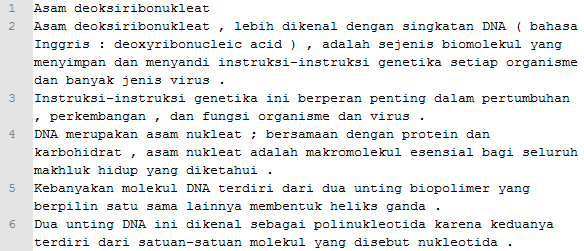
\includegraphics[width=1\linewidth]{pics/sen-split}
	\caption{Contoh hasil proses pemisahan kalimat}
	\label{fig:sen-split}
\end{figure}

%-----------------------------------------------------------------------------%
\section{Pemodelan Word Embedding}
%-----------------------------------------------------------------------------%
Pembentukan model \textit{word embedding} dilakukan dengan bantuan \textit{library}  Gensim-Word2Vec\footnote{https://radimrehurek.com/gensim/models/word2vec.html} yang tersedia untuk bahasa Python. Seperti yang disebutkan pada bagian \ref{word-embedding}, salah satu cara mengaplikasikan \textit{word embedding} adalah menggunakan prosedur \textit{word2vec}. \textit{Library} Gensim-Word2Vec adalah \textit{library} bahasa Python yang dapat digunakan untuk mengimplementasikan prosedur \textit{word2vec}. \textit{Library} tersebut diaplikasikan pada program Python yang memproses masukan berupa hasil pemisahan kalimat. Berikut adalah kode program tersebut.
\begin{lstlisting}[language=Python, caption={Pemodelan \textit{word embedding}}, label={kode-pemodelan-word-embedding}]
from gensim.models import word2vec

file = #file berisi kalimat-kalimat
sentences = []
for sentence in file:
	words = sentence.split()
	if (len(words) > 1):
		sentences.append(words)

model = word2vec.Word2Vec(sentences 
						, size = #panjang vektor
						, window = #ukuran window
						, min_count = #jumlah kata minimum
						)
model.save(model_name)
\end{lstlisting}
Kode \ref{kode-pemodelan-word-embedding} menerima masukan berupa \textit{list of} kalimat. Kemudian setiap kalimat ditokenisasi menjadi \textit{list of} kata. \textit{Word2vec} menerima \textit{list of list} kata untuk membentuk model \textit{word2embedding}. Kemudian, yang perlu dilakukan adalah mengatur parameter lain pada \textit{word2vec}, yaitu \textit{size} yang merupakan panjang dari vektor kata yang dibuat, \textit{window} adalah jumlah kata yang diprediksi dari suatu kata, \textit{min\_count} adalah panjang minimum dari \textit{list} kata yang dimasukkan.


%-----------------------------------------------------------------------------%
\section{Pembentukan T dan H} 
%-----------------------------------------------------------------------------%
Seperti yang telah dijelaskan pada bagian \ref{sec:pembentukanTdanH}, ada lima proses yang harus dilakukan. Pada bagian ini akan dijelaskan cara mengimplementasikan proses tersebut.
\begin{enumerate}
	\item Penghapusan kata-kata yang mengarah ke vandalisme\\
	Kode \ref{kode-vandal} menunjukkan proses penghapusan kata-kata yang mengarah pada kasus vandalisme. Kata-kata yang mengarah pada vandalisme tersebut terlebih dahulu didaftarkan dan disimpan dalam sebuah \textit{list}.
	\begin{lstlisting}[language=Python, caption={Penghapusan kata-kata yang mengarah ke vandalisme}, label={kode-vandal}]
	text = #teks yang sedang diproses
	vandal_words = #daftar kata-kata yang tergolong vandal
	
	for word in vandal_words: 
		text = text.remove(word)
	return text
	\end{lstlisting}	
	\item Pemasangan teks induk dan teks revisi\\
	Kode \ref{kode-pemasangan-teks} menunjukkan proses pemasangan kalimat. Setiap teks revisi dipasangkan dengan teks induknya yaitu teks dengan \textit{id} yang sama dengan \textit{parent id} pada teks revisi.
	\begin{lstlisting}[language=Python, caption={Pemasangan teks induk dan revisi}, label={kode-pemasangan-teks}]
	TH_pairs = []
	for article in file: #semua artikel dalam file
		for r in article: #semua teks revisi di artikel, kecuali teks pertama
			p_id = #parent_id
			TH_pairs.append([r, article[p_id]]) #ambil artikel induk
	return TH_pair
	\end{lstlisting}
	
	\item Penyesuaian paragraf\\
	Kode \ref{kode-penyesuaian-par} menunjukkan proses penyesuaian paragraf. Paragraf pada teks induk dan revisi terlebih dahulu diidentifikasi. Salah satu cara identifikasi adalah menggunakan tanda \textit{newline}. Untuk setiap paragraf di teks induk, pasangkan dengan salah satu paragraf yang sesuai di teks revisi. Pemasangan tersebut dilakukan secara terurut. Pada penelitian ini, paragraf kami anggap sesuai apabila paling tidak memiliki sebuah teks yang sama. 
	\begin{lstlisting}[language=Python, caption={Penyesuaian paragraf}, label={kode-penyesuaian-par}]
	def paragraph_alignment(parent_text, revisi_text) :	
		#inisialisasi pasangan paragraf
		par_pairs = []
		#pisahkan paragraf di teks induk
		parent_pars = parent_text.split(newline)
		#pisahkan paragraf di teks revisi
		revision_pars = revisi_text.split(newline)	
		
		i = 0
		j = 0
		while (i < len(parent_pars)): 
			moving_j = j
			while (moving_j < len(revision_pars) and i < len(psarent_pars)):
				if same_paragraph(revision_pars[i], parent_pars[moving_j]):
					#simpan pasangan paragraf yang sesuai
					par_pairs.append(parent_pars[moving_j], revision_pars[i])
					i++
					j = moving_j + 1
				moving_j++
			i++
		return par_pairs
	\end{lstlisting}
	
	\item Penyesuaian kalimat\\
	Kalimat-kalimat dari pasangan paragraf yang sesuai kemudian dibandingkan agar dapat diketahui kalimat mana yang sama antar kedua paragraf tersebut. Dua kalimat dianggap sama jika:
	\begin{itemize}
		\item Kedua kalimat sama persis
		\item Perbedaan antara dua kalimat hanya berupa keterangan tambahan menggunakan tanda kurung (). Contoh: "Asam Deoksiribonukleat (DNA) adalah ..." dan "Asam Deoksiribonukleat adalah ..."
		\item Perbedaan antara kedua kalimat hanya perbaikan kata-kata salah ejaan. Contoh: "Antropologi adalah salah satu cabang ilmu social ..." dan "Antropologi adalah salah satu cabang ilmu sosial ...". Untuk kasus ini, kata-kata salah ejaan diidentifikasi menggunakan algoritme Levenstein Distance \citep{Levenshtein_SPD66}. Dimana jika \textit{distance} yang diberikan lebih kecil dari 3, kata dianggap sama.
		\begin{lstlisting}[language=Python, caption={Levenstein Distance}]
	def levenshteinDistance(word_1, word_2):
		if len(word_1) > len(word_2):
			word_1, word_2 = word_2, word_1
			
		distances = range(len(word_1) + 1)
		for i, char_2 in enumerate(word_2):
			distances_ = [i+1]
			for j, char_1 in enumerate(word_1):
				if char_1 == char_2:
					distances_.append(distances[j])
				else:
					distances_.append(1 + min((distances[j], distances[j + 1], distances_[-1])))
			distances = distances_
		return distances[-1]
		\end{lstlisting}
		\item Kalimat hanya berbeda dari segi penggunaan huruf besar dan kecil
		\item Kalimat hanya berbeda dari segi penggunaan tanda baca
	\end{itemize}
	
	\item Pemasangan Kalimat\\
	Kelompok kalimat penambahan di teks induk dan kelompok kalimat pengurangan di teks revisi yang berada yang berada di antara kalimat yang sama dipasangkan sesuai dengan aturan berikut.
	\begin{itemize}
		\item Apabila jumlah kalimat yang dikurangi lebih banyak, kalimat pengurangan di posisi akhir (yang tidak mendapat pasangan) tidak akan digunakan.
		\item Apabila jumlah kalimat yang ditambahkan lebih banyak, kalimat tambahan  di posisi akhir dipasangkan dengan kalimat yang berada sebelum kalimat tersebut di dalam teks akhir. Hal ini  dilakukan dengan pertimbangan bahwa, sebuah kalimat yang ditambahkan bisa saja berupa rincian atau penjelas dari kalimat sebelumnya.
		\item Selebihnya, kalimat yang dikurangi dipasangkan dengan kalimat tambahan dengan urutan yang sesuai.
	\end{itemize}
	Kode \ref{kode-pemasangan-kalimat} menunjukkan implementasi dari aturan di atas.
	\begin{lstlisting}[language=Python, caption={Pemasangan kalimat}, label={kode-pemasangan-kalimat}]
	def T_H_pairing(sen_group_1, sen_group_2):
		pairs = []
		#aturan poin pertama
		if len(sen_group_1) > len(sen_group_2): 
			sen_group_1 = sen_group_1[:len(sen_group_2)] #potong kalimat yang berlebih
		#aturan poin kedua
		elif len(sen_group_2) > len(sen_group_1): 
			for i in range(len(sen_group_1) .. len(sen_group_2)-1):
				#pasangkan dengan kalimat sebelumnya
				pairs.append([sen_group_2[i], sen_group_2[i+1]])
		
		#aturan poin ketiga
		for i in range(0 .. min(len(sen_group_1), len(sen_group_2))):
			#pasangkan kalimat dengan posisi yang sesuai
			pairs.append([sen_group_1[i], sen_group_2[i]])
		return pairs	
	\end{lstlisting}
	Proses pemasangan belum berakhir, pasangan kalimat tersebut perlu ditentukan posisinya yaitu kalimat mana yang berperan sebagai T dan mana yang menjadi H. Untuk menentukan hal tersebut kami hanya menggunakan perbandingan panjang kalimat (dihitung dari jumlah kata) sebagai pertimbangan. Kalimat yang lebih panjang akan menjadi T, selebihnya menjadi H. Terakhir, pasangan T dan H diberi pelengkap yaitu komentar penulis yang diambil dari komentar pada teks revisi.

\end{enumerate}
%-----------------------------------------------------------------------------%
\section{Ekstraksi Fitur}
%-----------------------------------------------------------------------------%
Pada bagian ini akan dijelaskan ekstraksi fitur yang dilakukan pada kedua \textit{view}. Masing-masing \textit{view} diekstrak dengan cara yang berbeda. 

\subsection{Ekstraksi Fitur View Pertama}
Fitur utama dari \textit{view} pertama adalah fitur \textit{word embedding} masing-masing teks T dan H. Untuk mengetahui vektor \textit{word embedding} masing-masing kata, diperlukan model \textit{word embedding} yang sebelumnya telah dibuat. Kode {kode-ekstraksi-WE} menunjukkan proses ekstraksi fitur \textit{word embedding}.
\begin{lstlisting}[language=Python, caption={Ekstraksi Fitur \textit{word embedding}}, label={kode-ekstraksi-WE}]
from gensim.models import word2vec
vector_null = #vektor default [0, 0, ...]

def sentence_to_vec (sentence):
	vec = []
	model = word2vec.Word2Vec.load(model_name) #nama model
	words = sentence.split()
	for word in words:
		try:
			vec.append(model[word].tolist()) #mencari vektor kata menggunakan model
		except:
			vec.append(vector_null) #jika kata tidak pernah dimasukkan ke model, gunakan vektor default
	return vec
\end{lstlisting}
Fitur yang terbentuk adalah sebuah vektor dengan elemen berupa \textit{word embedding}  dari semua penyusun teks. Apabila kata yang penyusun teks tersebut tidak ada di dalam model \textit{word embedding}, kata akan diganti dengan vektor \textit{default}. Panjang vektor yang digunakan harus sama, agar memiliki panjang yang sama, kami melakukan \textit{padding} terhadap seluruh vektor kalimat T dan H. \textit{Padding} adalah proses penambahan elemen pada vektor yang panjangnya tidak mencapai batas yang ditentukan. \textit{Padding} dilakukan dengan menambahkan vektor \textit{null} di bagian akhir vektor yang panjangnya masih di bawah batas. Semua vektor di-\textit{padding} hingga panjangnya mencapai panjang vektor kalimat dengan kata terbanyak.  

Pada arsitektur RNN kedua, ada 6 buah fitur tambahan yang perlu diimplementasikan, yaitu:
\begin{enumerate}	
	\item Rata-rata \textit{similarity} dari pasangan kelompok kata yang tidak bersesuaian di T dan H kecuali yang berpasangan dengan kelompok kosong. 		
	\item Nilai dalam rentang 0 hingga 1 yang menggambarkan jumlah pasangan kelompok kata di T yang berpasangan dengan kelompok kosong ([]) di H.
	\item Nilai dalam rentang 0 hingga 1 yang menggambarkan jumlah pasangan kelompok kata di H yang berpasangan dengan kelompok kosong ([]) di T. 
	\item Nilai dalam rentang 0 hingga 1 yang merepresentasikan jumlah kata yang sesuai dari T dan H. 
	\item Nilai dalam rentang 0 hingga 1 yang merepresentasikan panjang LCSS dari T dan H. 
	\item Nilai yang merepresentasikan kebenaran bahwa T dan H diawali kata yang sama. 
\end{enumerate}	
Kode \ref{kode-fitur-tambahan} menunjukkan implementasi dari fitur tambahan di atas. 
\begin{lstlisting}[language=Python, caption={Penambahan fitur arsitektur RNN kedua}, label={kode-fitur-tambahan}]
#masukan adalah kalimat T dan H
def addOtherFeatures(text, hipo):
	OtherFeature = []
	T = text.split()
	H = hipo.split()		
	(same, diff)  = calculate_diff(T, H)
	feature1 = avg(diff) #mencari rata-rata nilai dalam list 'diff' kecuali yang bernilai 1 dan -1
	feature2 = sigmoid(count(-1, diff)) #hitung jumlah -1 di 'diff'
	feature3 = sigmoid(count(1, diff)) #hitung jumlah 1 di 'diff'
	feature4 = (2 * same) / (len(T) + len(H))
	feature5 = (2 * (LCSS(T, H)) / (len(T) + len(H))	
	feature6 = T[0] == H[0] ? 1 : 0
	OtherFeature = [feature1, feature2, feature3, feature4, feature5, feature6]
	return OtherFeature
\end{lstlisting}
\noindent Fungsi LCSS yang digunakan adalah LCSS pada umumnya. Sedangkan,  untuk menghitung nilai \textit{similarity}, digunakan fungsi \textit{n\_similarity()} yang disediakan olen Gensim Word2vec, yaitu fungsi yang menghitung \textit{cosine similarity} dari dua buah \textit{list} kata. Pada kode \ref{kode-fitur-tambahan-2}, ditampilkan cara menghitung kemunculan kata bersesuaian, mengelompokkan kata, dan menghitung \textit{similarity} kelompok kata tersebut.

\begin{lstlisting}[language=Python, caption={Perhitungan \textit{similarity} kelompok kata}, label={kode-fitur-tambahan-2}]
from gensim.models import word2vec

def calculate_diff(T, H):
	model = #load model word embedding
	same = 0 #inisalisasi jumlah kata sesuai
	diff = group_1 = group_2 = [] #inisialisasi hasil, kelompok perubahan kata di T, dan kelompok perubahan kata di H
	#membatasi akhir dan awal kalimat
	Tword = ['<start>'] + T + ['<end>']
	Hword = ['<start>'] + H + ['<end>']	
	s = s_new = 0
	for i, t in enumerate(Tword):
		found = False
		moving_s = s
		while (moving_s < len(Hword)): 
			if (t == Hword[moving_s]):
				same += 1
				found = True
				s_new = moving_s		  
				break
			else:
				moving_s = moving_s + 1					
			
		if (found == False):
			group_1.append(Tword[i])
		else:
			for k in range(s+1, s_new):
				group_2.append(Hword[k])		
			#kelompok kata T kosong
			if (len(group_2) != 0 and len(group_1)==0):
				diff.append(-1)
			#kelompok kata H kosong
			elif (len(group_2) == 0 and len(group_1)!=0):
				diff.append(1)
			else:
				#similarity antar kelompok kata
				diff.append(model.n_similarity(group_1, groupt_2))
			group_1 = group_2 = []
		s = s_new	  
	return (same, diff)	
\end{lstlisting}
\noindent Fungsi di atas akan menerima masukan dua buah teks dan mengembalikan nilai \textit{similarity} dari tiap kelompok perubahan kata pada teks. Hasil yang diberikan berupa jumlah kata bersesuaian antara kedua teks dan daftar nilai \textit{similarity}, seperti \textit{[similarity 1, similarity 2, ...]}. 

\subsection{Ekstraksi Fitur View Kedua}
Program Weka GUI\footnote{http://www.cs.waikato.ac.nz/ml/weka/} digunakan untuk menentukan fitur pada \textit{view} kedua. Fitur untuk \textit{view} kedua berupa jumlah kemunculan unigram, bigram, dan trigram terbanyak yang muncul pada komentar penulis dari seluruh data. Oleh karena itu, sebelum mendaftarkan apa saja fitur view kedua, frekuensi kemunculan N-gram pada data terlebih dahulu harus dibuat. Kemudian, N-gram diurutkan berdasarkan frekuensinya, beberapa N-gram terbanyak akan dipilih sebagai fitur \textit{view} kedua. Akan tetapi, jumlah kemunculan N-gram pada daftar tersebut belum tentu akan menghasilkan kombinasi fitur yang paling baik. Oleh karena itu, kami menggunakan fitur \textit{select attribute} pada Weka GUI dengan metode \textit{genetic search} untuk memilih kombinasi fitur terbaik.


%-----------------------------------------------------------------------------%
\section{Co-training} \label{sec:cotrain}
%-----------------------------------------------------------------------------%
Co-training akan berjalan dalam beberapa iterasi hingga mencapai \textit{stopping condition}. Pada penelitian ini, \textit{stopping condition} yang digunakan adalah ketika kedua \textit{classifier} tidak mengklasifikasikan data dengan sesuai. Sedikit variasi untuk kondisi tersebut, algoritme Co-training akan berhenti ketika kedua \textit{classifier} tidak mampu menyepakati satu pun label yang sama dalam \textit{n} iterasi berurutan.
\begin{lstlisting}[caption={Algoritme Co-training yang akan digunakan}, label={fig:Co-training}]
Masukan:
L = data berlabel 
U = data tidak berlabel

U' = sejumlah k data dari U
iterasi_gagal = 0
Selama iterasi_gagal < n:
	Latih classifier h1 dengan data L dari view pertama
	Latih classifier h2 dengan data L dari view kedua
	Klasifikasi U' dengan h1 dapatkan U1'
	Klasifikasi U' dengan h2 dapatkan U2' 
	Ambil data terbaik dari U1' dan U2' 
		Jika jumlah data terbaik = 0, iterasi_gagal++
		Jika jumlah data terbaik > 0, iterasi_gagal = 0
	Ambil k data dari U untuk menggantikan isi U'

\end{lstlisting}
Kode \ref{fig:Co-training} menunjukkan algoritme Co-training yang diajukan untuk penelitian ini. 
Data hasil klasifikasi terbaik pada setiap iterasi adalah data yang diklasifikasikan oleh masing-masing \textit{classifier} yang menghasilkan label yang sama dan dengan tingkat kepercayaan (lihat bagian \ref{ssl-ssl}) untuk label tersebut melebihi batas yang ditentukan. Semakin tinggi tingkat kepercayaan sebuah kelas terpilih menunjukkan bahwa \textit{classifier} semakin yakin dalam melakukan klasifikasi. Sedangkan, untuk tetap menjaga keseimbangan data berlabel, jumlah data hasil klasifikasi yang diambil akan diperhatikan perbandingannya. 

